\documentclass{article}
\usepackage[utf8]{inputenc}
\usepackage{indentfirst}
\usepackage{titling}
\usepackage{geometry}
\usepackage{graphicx}
\graphicspath{ {./Images/} }
\usepackage[shortlabels]{enumitem}
\usepackage{fancyhdr}
\usepackage{ulem}
\usepackage[dvipsnames]{xcolor}
\usepackage{amssymb}
\usepackage{listings}
\usepackage{color}

\definecolor{dkgreen}{rgb}{0,0.6,0}
\definecolor{gray}{rgb}{0.5,0.5,0.5}
\definecolor{mauve}{rgb}{0.58,0,0.82}

\lstset{frame=tb,
  language=Java,
  aboveskip=3mm,
  belowskip=3mm,
  showstringspaces=false,
  columns=flexible,
  basicstyle={\small\ttfamily},
  numbers=none,
  numberstyle=\tiny\color{gray},
  keywordstyle=\color{blue},
  commentstyle=\color{dkgreen},
  stringstyle=\color{mauve},
  breaklines=true,
  breakatwhitespace=true,
  tabsize=3
}

\def\ojoin{\setbox0=\hbox{$\bowtie$}%
  \rule[-.02ex]{.25em}{.4pt}\llap{\rule[\ht0]{.25em}{.4pt}}}
\def\leftouterjoin{\mathbin{\ojoin\mkern-5.8mu\bowtie}}
\def\rightouterjoin{\mathbin{\bowtie\mkern-5.8mu\ojoin}}
\def\fullouterjoin{\mathbin{\ojoin\mkern-5.8mu\bowtie\mkern-5.8mu\ojoin}}

\renewcommand\maketitlehooka{\null\mbox{}\vfill} %para centralizar verticalmente
\renewcommand\maketitlehookd{\vfill\null}
\pagestyle{fancy}
\fancyhf{}
\rfoot{\thepage}
\lfoot{ 
\includegraphics[scale=0.01]{UA.jpg} José Mendes 107188 LEI}
\geometry{
  a4paper,
  headheight=4cm,
  top=5.5cm,
  bottom=4.5cm,
  footskip=4cm
}


\title{Introdução à Engenharia de Software}
\author{José Mendes 107188}
\date{2023/2024}

\begin{document}


\begin{titlepage}
    \maketitle
    \begin{center}
        
\includegraphics[scale=0.4]{UA.png}
    \end{center}
    \thispagestyle{empty} %remove o count da pagina
\end{titlepage}

\pagebreak

\section{Maven}

\subsection{O que é o Maven?}

É uma \textbf{ferramenta de gestão de projetos}, que inclui:
\begin{itemize}
  \item Um \textbf{project object model} (POM) que descreve o projeto;
  \item Um conjunto de \textbf{standards};
  \item Um \textbf{lifecycle} do projeto;
  \item Um sistema de gestão de \textbf{dependências};
  \item Lógica para \textbf{executar plugins} em \textbf{fases} específicas
  do ciclo de vida.
\end{itemize}

Convenção sobre configuração (layout do projeto é padronizado).

\subsection{Layout de Diretórios Padronizado}

\begin{flushleft}
  \textbf{POM} - Contém uma descrição completa do projeto de como
  construir o projeto.

  \vspace{2mm}

  \textbf{src} - Diretório que contém todo o código fonte para construir
  o projeto, o seu site, \dots

  \vspace{2mm}

  \textbf{target} - Diretório que contém os resultados da construção,
  tipicamente um JAR ou WAR, juntamente com os ficheiros intermedios.
\end{flushleft}

\subsection{POM}

Maven é baseado no conceito de um \textbf{Project Object Model} (POM).
Este é um ficheiro XML, que está sempre localizado no diretório base do projeto
como \textbf{pom.xml} (os users definiram POMs que estendem o Super POM).

O POM contém informação sobre o projeto e vários detalhes de configuração
usados pelo Maven para construir o projeto.

O POM é declarativo, não necessita de detalhes de procedimento.

\subsubsection{Estrutura do POM}

\begin{flushleft}
  O POM contém 4 categorias de descrição e configuração:
  
  \begin{itemize}
    \item Informação geral do projeto, isto é, informação human-readable;
    \item Configuração do build, que pode incluir, adicionar plugins,
    afixar plugins objetivo ao ciclo de vida;
    \item Ambiente de construção, que descreve o ambiente "familiar" em que o Maven está;
    \item Relações POM, isto é, coordenadas, herança, agregação, dependências.
  \end{itemize}
\end{flushleft}

\pagebreak

\subsection{Coordenadas Maven}

As coordenadas definem o lugar único do projeto no universo Maven.
São compostas por 3 partes: \textbf{$<$groupId$>$}, \textbf{$<$artifactId$>$} e
\textbf{$<$version$>$} (The Maven trinity!).

\vspace{2mm}

As versões de um projeto são usadas para agrupar e ordenar lançamentos:

\[ <major\_version>.<minor\_version>.<incremental\_version>-<qualifier> \]

\begin{flushleft}
  \textbf{Exemplo:} 1.0.0-SNAPSHOT ou 1.2.3-alpha-2
\end{flushleft}

Se o qualifier contiver a palavra chave SNAPSHOT, então o Maven
vai expandir este token para uma data e hora convertida para o formato UTC.

\vspace{2mm}

\begin{flushleft}
  \begin{itemize}
    \item \textbf{groupId} - Nome da empresa, organização, equipa, \dots,
    normalmente usando a convenção de nomes de domínio invertidos (reverse URL naming, ex: org.apache.maven);

    \item \textbf{artifactId} - Nome único do projeto dentro do groupId;
    
    \item \textbf{version} - Versão do projeto;
    \item \textbf{packaging} - Tipo de empacotamento do projeto (jar (default), war, \dots);
    \item \textbf{classifier} - Classificador opcional para distinguir artefactos
  \end{itemize}

  \vspace{2mm}

  \textbf{Nota:} As coordenadas Maven identificam unicamente um projeto.
\end{flushleft}

\subsection{Ciclo de Vida Maven}

Um ciclo de vida é uma sequência organizada de fases,
que dão ordem a uma sequência de objetivos.
Estes objetivos são empacotados em plugins que estão ligados
as fases.

\begin{center}
  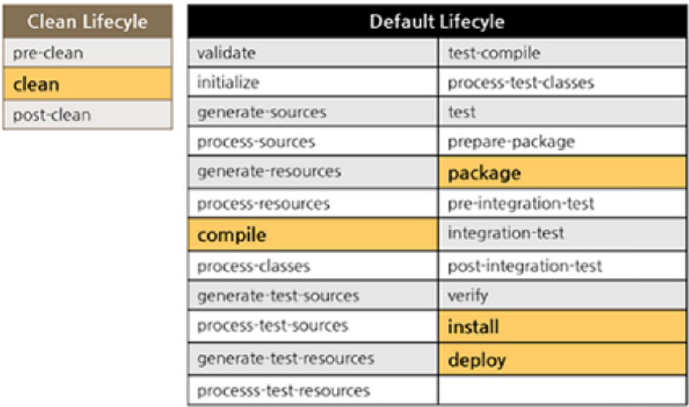
\includegraphics[scale=0.5]{1}
\end{center}

Chamar uma fase específica num ciclo de construção, vai executar
todas as fases anteriores a essa fase.

\pagebreak

\begin{center}
  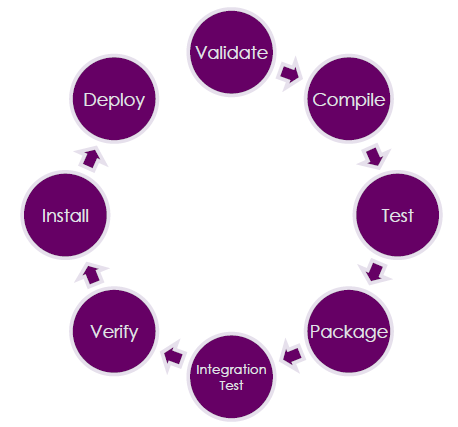
\includegraphics[scale=0.5]{2}
\end{center}

\begin{flushleft}
  \begin{enumerate}
    \item \textbf{Validate} - Valida que a estrutura do projeto está correta.
    (ex: verifica se todas as dependências foram transferidas e estão disponíveis
    no repositório local);

    \item \textbf{Compile} - Compila o código fonte, converte os ficheiros
    \textbf{.java} em \textbf{.class}, e armazenando-os no diretório \textbf{target/classes};

    \item \textbf{Test} - Corre testes unitários para o projeto;
    \item \textbf{Package} - Empacota o código compilado num formato distribuível
    como \textbf{JAR} ou \textbf{WAR};

    \item \textbf{Integration Test} - Corre testes de integração para o projeto;
    \item \textbf{Verify} - Corre verificações para verificar que o projeto é válido
    e que cumpre os critérios de qualidade;

    \item \textbf{Install} - Instala o código empacotado
    no repositório Maven local, para uso como dependência noutros projetos locais;

    \item \textbf{Deploy} - Copia o pacote final de código para o repositório
    remoto para partilha com outros developers e projetos.
  \end{enumerate}
\end{flushleft}

\subsection{Ciclo de Vida de Construção}

O processo para contruir e distribuir um projeto. Consiste
em vários passos designados por \textbf{fases}.

Algumas fases default são:
\begin{itemize}
  \item \textbf{validate}
  \item \textbf{compile}
  \item \textbf{test}
  \item \textbf{package}
  \item \textbf{deploy}
\end{itemize}

\pagebreak

\subsection{Goals e Plugins}

Os Goals são operações fornecidas pelas ferramentas Maven.

Cada fase é uma sequência de Goals, em que cada Goal é responsável
por uma tarefa específica. Quando corremos uma fase, todos os Goals
ligados a essa fase são executados, na ordem em que estão definidos.

\begin{flushleft}
  Algumas Maven Plugins:
  \begin{itemize}
    \item resources
    \item compiler
    \item surefire
    \item jar, war
  \end{itemize}
\end{flushleft}

\subsection{Arquétipos (Archetypes)}

Um Archetype é um template para um projeto Maven, que pode ser usado para
criar um novo projeto rapidamente.

\begin{flushleft}
  \textbf{Exemplo:} \textit{maven-archetype-quickstart} ou \textit{maven-archetype-webapp}
\end{flushleft}

Users podem criar os seus próprios Archetypes e publicá-los através de catálogos.

\subsection{Gestor de Dependências}

Uma \textbf{dependência} de um projeto é uma biblioteca da qual
o projeto depende. Adicionar uma dependência ao projeto é simples,
basta adicionar a dependência ao POM. O Maven vai automaticamente
procurar a dependência no repositório local, e se não encontrar,
vai procurar no repositório remoto e transferi-la.

\begin{center}
  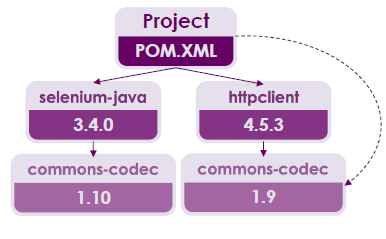
\includegraphics[scale=0.6]{3}
\end{center}

\pagebreak

\section{Git e GitHub}

\subsection{Sistemas de Controlo de Versões}

Um sistema de controlo de versões (também conhecido como sistema de controlo de código fonte) faz o seguinte:
\begin{itemize}
  \item Mantém várias (antigas e novas) versões de tudo (não só código fonte);
  \item Pede por comentários quando se fazem alterações;
  \item Permite "check-in" e "check-out" de ficheiros para saber
  em que ficheiros outras pessoas estão a trabalhar;
  \item Mostra as diferenças entre versões;
\end{itemize}

\subsubsection{Vantagens}

\begin{flushleft}
  \textbf{Ao trabalhar sozinho:} Fornece uma "máquina do tempo" para
  voltar atrás para uma versão anterior, e fornece um bom suporte 
  de diferentes versões do mesmo projeto.

  \vspace{2mm}

  \textbf{Ao trabalhar em equipa:} Simplifica muito trabalhar em concurrencia,
  dando "merge" de alterações feitas por diferentes pessoas.
\end{flushleft}

\subsection{o que é Git e GitHub}

\begin{center}
  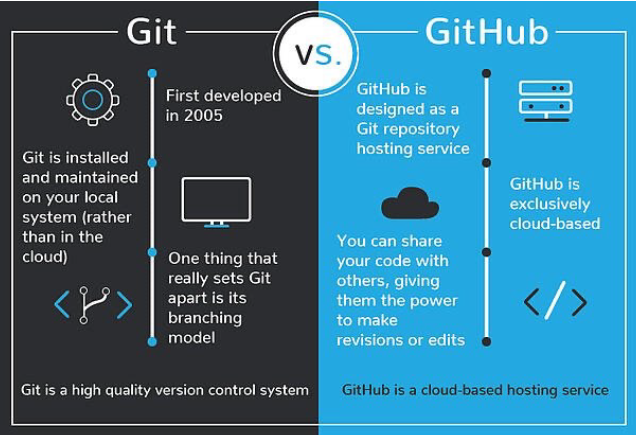
\includegraphics[scale=0.5]{4}
\end{center}

Quando fazemos "git init" num diretório de um projeto, ou quando fazemos
"git clone" de um projeto existente, o Git cria um repositório (.git).

Em qualquer momento, podemos fazer um "snapshot" de tudo
no dirétorio do projeto e guardar este no repositório.
Este "snapshot" é chamado de \textbf{commit object}.

\pagebreak

Um \textbf{commit} ocorre quando fazemos alterações que estão
prontas para serem guardadas no repositório.

Quando realizamos um commit, o Git guarda um \textbf{commit object}:
\begin{itemize}
  \item Um estado completo do projeto, incluindo todos os ficheiros;
  \item O primeio não possui pai;
  \item Normalmente, pegamos num commit object, fazemos alterações,
  e criamos um novo commit object, pelo que a maior parte dos commit objects
  têm apenas um pai;
  \item Quando fazemos \textbf{merge} de dois commit objects,
  forma um commit object com dois pais.
\end{itemize}

Pelo que, os commit objects formam uma \textbf{DAG} (Directed Acyclic Graph).
O Git é tudo sobre usar e manipular este grafo.

\subsubsection{Mensagem de Commit}

Os commits são "baratos" pelo que os devemos fazer com frequência, e com
mensagens descritivas sobre o que foi alterado. Devem ter apenas uma linha.

Como não devemos dizer muito numa linha, devemos fazer vários commits.

\begin{center}
  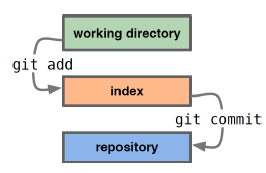
\includegraphics[scale=0.6]{5}
\end{center}

\subsection{Manter simples}

\begin{center}
  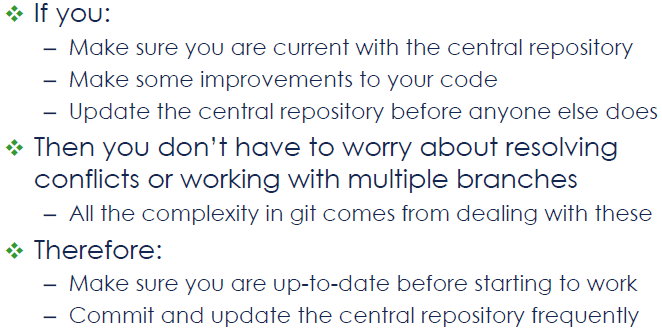
\includegraphics[scale=0.6]{6}
  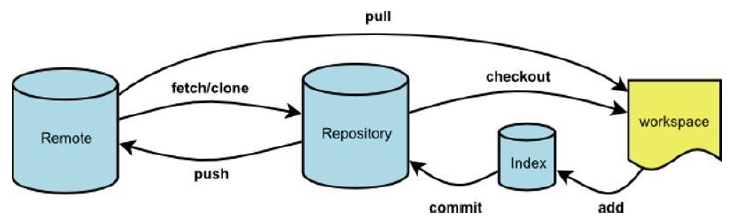
\includegraphics[scale=0.6]{7}
\end{center}

\end{document}